\documentclass[12pt,a4paper]{report}
\usepackage[hmargin=2cm,vmargin=3.5cm,bmargin=2cm]{geometry}
\usepackage[utf8]{inputenc}
\usepackage[portuguese]{babel}
\usepackage[T1]{fontenc}
\usepackage{amsmath}
\usepackage{amsfonts}
\usepackage{amssymb}
\usepackage{makeidx}
\usepackage{graphicx}
\usepackage{listings}
\usepackage{indentfirst}
\usepackage[pdftex]{hyperref}
\usepackage{csvsimple}
\usepackage{color}
\usepackage{mathtools}
\usepackage{float}

% Headers and Footers
\usepackage{fancyhdr}

\addto\captionsportuguese{\renewcommand{\chaptername}{}}

\definecolor{mygreen}{rgb}{0,0.6,0}
\definecolor{mygray}{rgb}{0.5,0.5,0.5}
\definecolor{mymauve}{rgb}{0.58,0,0.82}

\lstset{ %
  backgroundcolor=\color{white},   % choose the background color; you must add \usepackage{color} or \usepackage{xcolor}
  basicstyle=\footnotesize,        % the size of the fonts that are used for the code
  breakatwhitespace=false,         % sets if automatic breaks should only happen at whitespace
  breaklines=true,                 % sets automatic line breaking
  captionpos=b,                    % sets the caption-position to bottom
  commentstyle=\color{mygreen},    % comment style
  deletekeywords={...},            % if you want to delete keywords from the given language
  escapeinside={\%*}{*)},          % if you want to add LaTeX within your code
  extendedchars=true,              % lets you use non-ASCII characters; for 8-bits encodings only, does not work with UTF-8
  frame=single,                    % adds a frame around the code
  keywordstyle=\color{blue},       % keyword style
%  language=Octave,                 % the language of the code
  morekeywords={*,...},            % if you want to add more keywords to the set
  numbers=left,                    % where to put the line-numbers; possible values are (none, left, right)
  numbersep=5pt,                   % how far the line-numbers are from the code
  numberstyle=\tiny\color{mygray}, % the style that is used for the line-numbers
  rulecolor=\color{black},         % if not set, the frame-color may be changed on line-breaks within not-black text (e.g. comments (green here))
  showspaces=false,                % show spaces everywhere adding particular underscores; it overrides 'showstringspaces'
  showstringspaces=false,          % underline spaces within strings only
  showtabs=false,                  % show tabs within strings adding particular underscores
  stepnumber=2,                    % the step between two line-numbers. If it's 1, each line will be numbered
  stringstyle=\color{mymauve},     % string literal style
  tabsize=2,                       % sets default tabsize to 2 spaces
  title=\lstname                   % show the filename of files included with \lstinputlisting; also try caption instead of title
}


%\begin{itemize}
%\item A saída deve estar em ordem crescente (o elemento da saída não pode ser menor do que o seu antecessor de acordo com o critério adotado para ordenação);
%\item A saída é uma permutação (reordenação) da entrada;
%\end{itemize}
	
%\section{Algoritmos $\mathbf{O(n^2)}$}
%\subsection{Bubble Sort}

%\begin{lstlisting}[language=C++]
%\end{lstlisting}

%\begin{figure}[H]
%\includegraphics[width=\textwidth]{Imagens/bubble.png}
%\caption{Bubble Sort para diversos formatos de vetores}
%\end{figure}

%\begin{table}[H]
%\caption{Tabela dos tempos para os vetores de melhores e piores casos}
%\begin{center}
%\begin{tabular}{|c|c|c|c|c|c|}
%\hline 
%Caso & Bubble Sort (us) & Insertion Sort (us) & Merge Sort (us) & Heap Sort (us) & Quick Sort (us) \\ 
%\hline
%Melhor & 0,86	& 0,84 & 8,49 & 1,99 & 2,61 \\
%\hline 
%Pior & 24,97 & 24,56 & 8,97 & 7,73 & 15,8 \\
%\hline
%\end{tabular}
%\end{center}
%\end{table}


% Headers and Footers
\pagestyle{fancy} % fancy style
\lhead{\rightmark} % left header
\rhead{\leftmark} % right header
\lfoot{} % left footer
\cfoot{\textbf{\thepage}} % central footer
\rfoot{} % right footer
% Headers and Footers

\makeindex

% define the title
\author{Leandro Souza da  Silva - RA: 191082 \\ Luís Felipe Mattos - RA: 107822}
\title{MO655 - Comunicação em Datacenters}
%\date{}
\begin{document}

% generates the title
\maketitle

% insert the table of contents
\tableofcontents

\chapter{Introdução}

Com o crescimento da demanda dos usuários por poder computacional e armazenamento, cada vez mais as grandes empresas estão investindo em estruturas próprias de datacenters. Esta estrutura inclui tanto os computadores em si, os discos de armazenamento e os racks como também inclui a própria sala que ficarão estes racks. Estas salas devem tem uma arquitetura própria, como por exemplo, o piso elevado, sistema de refrigeração e circulação de ar. Um exemplo por ser visto na figura \ref{dc_overview}.\\

\begin{figure}[H]
\centering
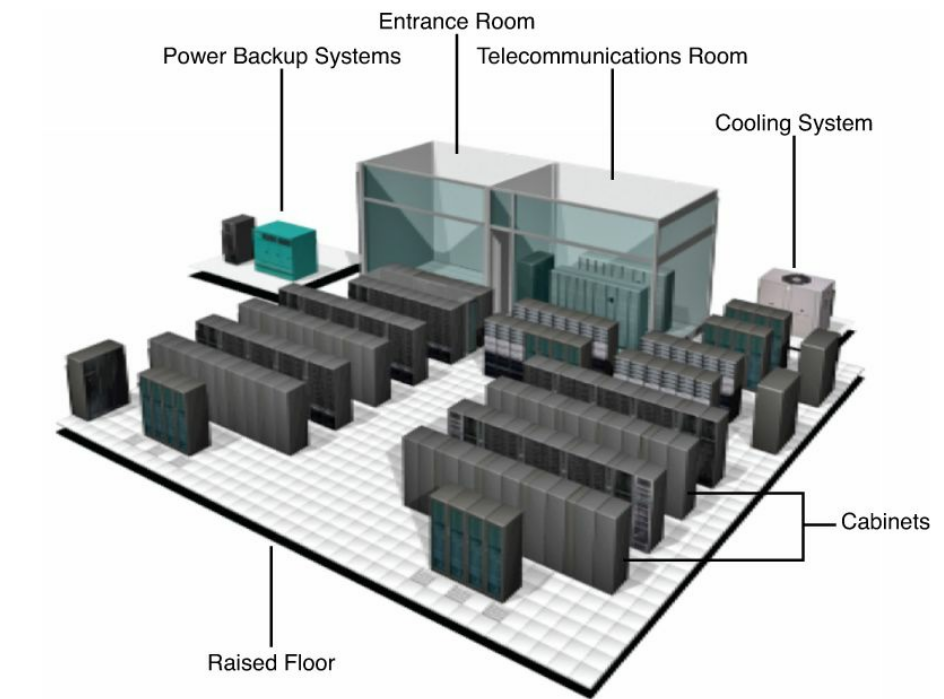
\includegraphics[width=.7\textwidth]{imagens/datacenter.png}
\caption{Visão geral de um Datacenter}
\label{dc_overview}
\end{figure}

Além da estrutura física, a parte computacional, principalmente relacionada à comunicação interna e externa do datacenter possui alguns requisitos básicos para que possa oferecer um serviço de qualidade para os usuários. Estes requisitos são citados a seguir:\\

\begin{itemize}
\item Escalabilidade
\item Tolerância a Falhas
\item Latêcia
\item Capacidade da Rede
\item Virtualização
\end{itemize}

A seguir, os requisitos citados serão mais detalhados.\\

\section{Requisitos de Rede}

\subsection{Escalabilidade}
O sistema deve ser construido de tal forma que seja possível haver uma expansão, caso a demanda aumente. Este requisito diz respeito tanto ao hardware como ao software. Para o hardware, a estrutura das máquinas deve permitir que o sistema seja melhorado e também deve haver espaço físico para a inclusão de novas máquinas. Atualmente, existem alguns sistemas modulares que possuem uma fácil integração de novos módulos.\\

Um exemplo é a utilização de datacenters em containers, cada container possui um sistema completo com refrigeração própria e é facilmente transportado. Com isso, pode-se expandir facilmente uma estrutura de um datacenter. Um exemplo de container pode ser visto na figura \ref{dc_container}.\\

\begin{figure}[H]
\centering
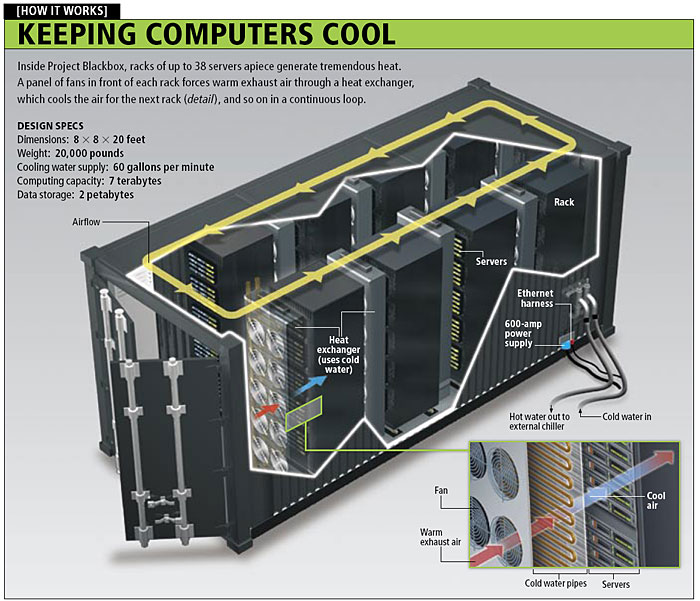
\includegraphics[width=.7\textwidth]{imagens/container_dc.jpg}
\caption{Datacenter em container}
\label{dc_container}
\end{figure}

\subsection{Tolerância a Falhas}
O sistema deve ser capaz de prevenir e corrigir falhas. Por causa disso, a maioria dos sistemas de datacenters possuem redundâncias em quase todos aspectos do datacenter. Existem backups dos dados dos usuários, a comunicação interna é feita de modo que existam vários caminhos possíveis da fonte para o destino e além disso, alguns datacenters possuem backups em outros datacenters. Apesar disso, existe o custo de manter estas cópias atualizadas.\\

Mais a frente falaremos um pouco mais sobre as redundâncias dos caminhos de comunicação interna dos datacenters, tanto relacionados à topologia como relacionado aos protocolos de comunicação e roteamento.\\

\subsection{Latêcia}
Um dos principais desafios dos datacenters é possuir baixa latência, assim, a performance do sistema como um todo se mantém em um nível aceitável pelos usuários. Para isso, a topologia é muito importante, uma vez que quanto menor o caminho entre a fonte e o destino, menor a latência. Porém, outro fator que influencia muito a latência é o nível de congestionamento da rede, mais a frente iremos tratar sobre os protocolos e como estes controlam o nível de congestionamento da rede.\\

\subsection{Capacidade da Rede}
A capacidade da rede está quase que diretamente ligada à latência, quanto maior a capacidade da rede, menor a latência. O requisito é que a capacidade da rede seja suficiente para que atinja a demanda de forma que o desempenho e a qualidade de serviços não sejam afetados, independente da quantidade de usuários.\\

\subsection{Virtualização}
Outro requisito é a virtualização. Este requisito é relacionado à escalabilidade, onde permite que haja uma capacidade elástica da rede e além disso, que o sistema seja capaz de mover sistemas virtualizados de uma máquina física para outra, sem que haja problemas de compatibilidade. Isso só é possível com a virtualização, que executa o mesmo sistema em cima da camada de hardware de modo transparente para os usuários.\\

\chapter{Motivação}

O crescimento da demanda dos usuários tem sido exponencial nos últimos anos, o gráfico da figura \ref{consumo}. Com isso, cada vez mais as empresas precisam investir na expansão e atualização dos datacenters para acompanhar a demanda. A figura \ref{servidores} mostra o crescimento do número de racks com servidores entre 2011 e 2013 no leste do Estados Unidos.\\

\begin{figure}[H]
\centering
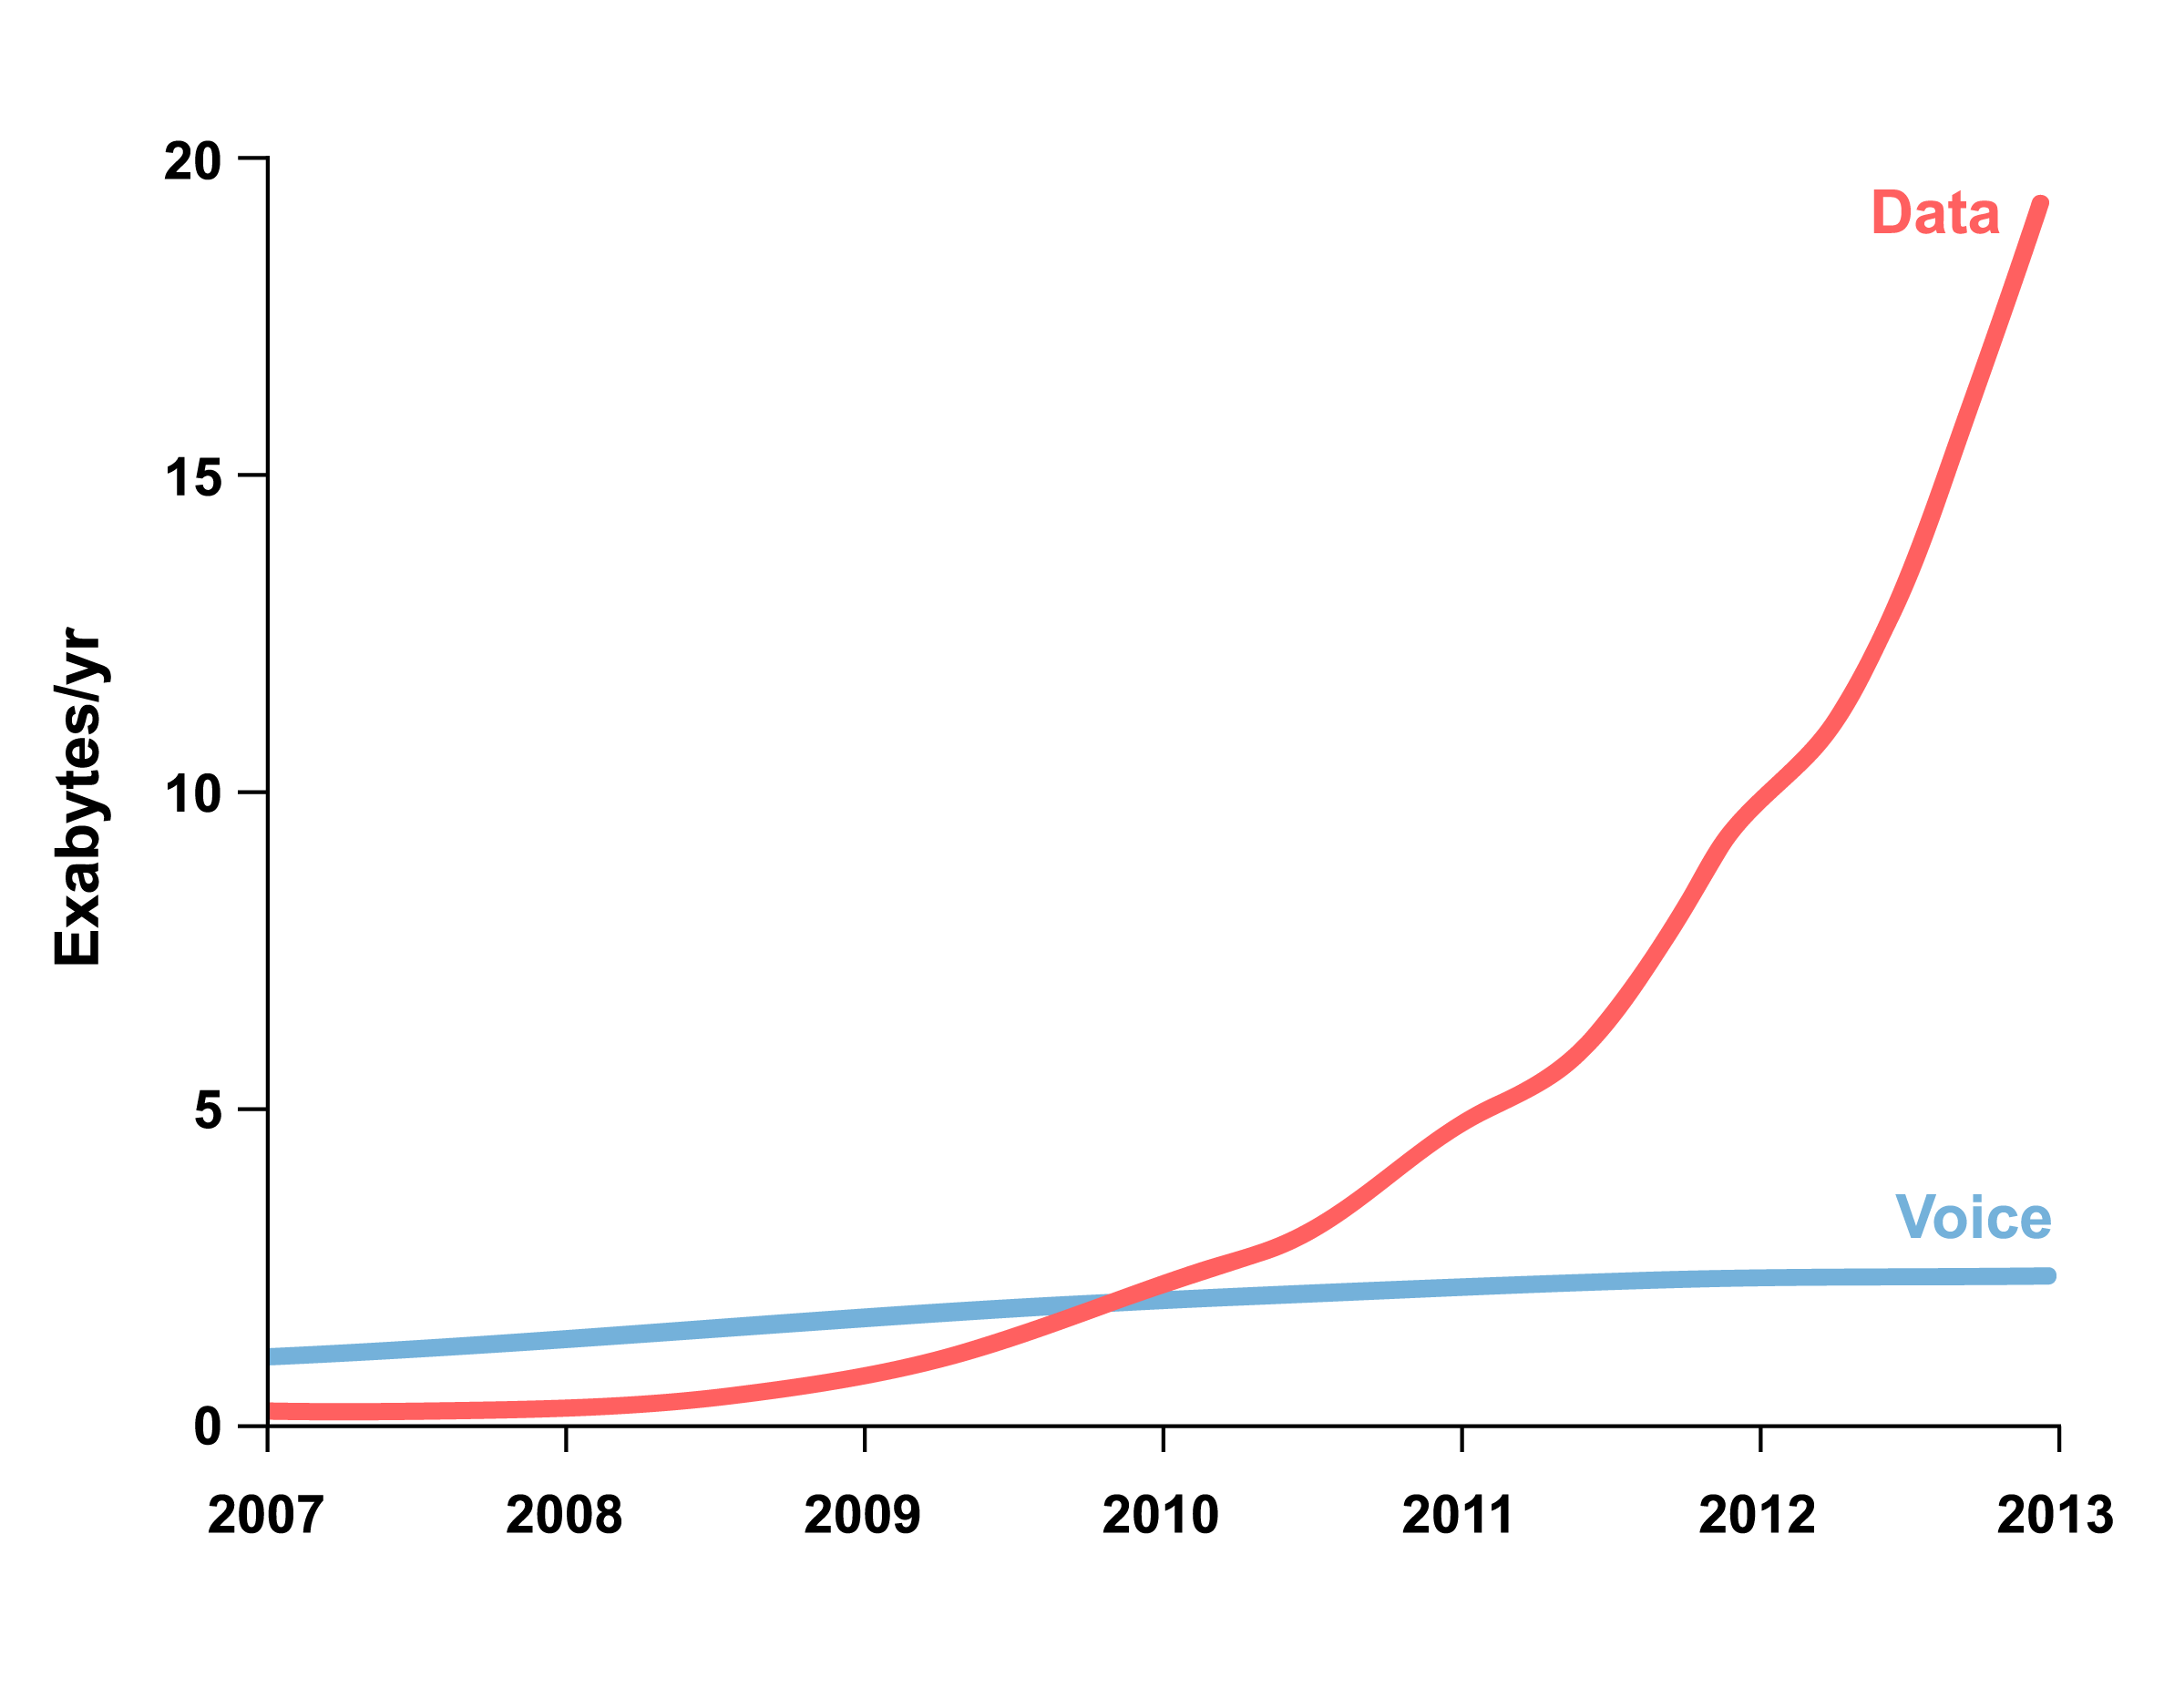
\includegraphics[width=.7\textwidth]{imagens/consumo.png}
\caption{Crescimento do consumo de dados}
\label{consumo}
\end{figure}

\begin{figure}[H]
\centering
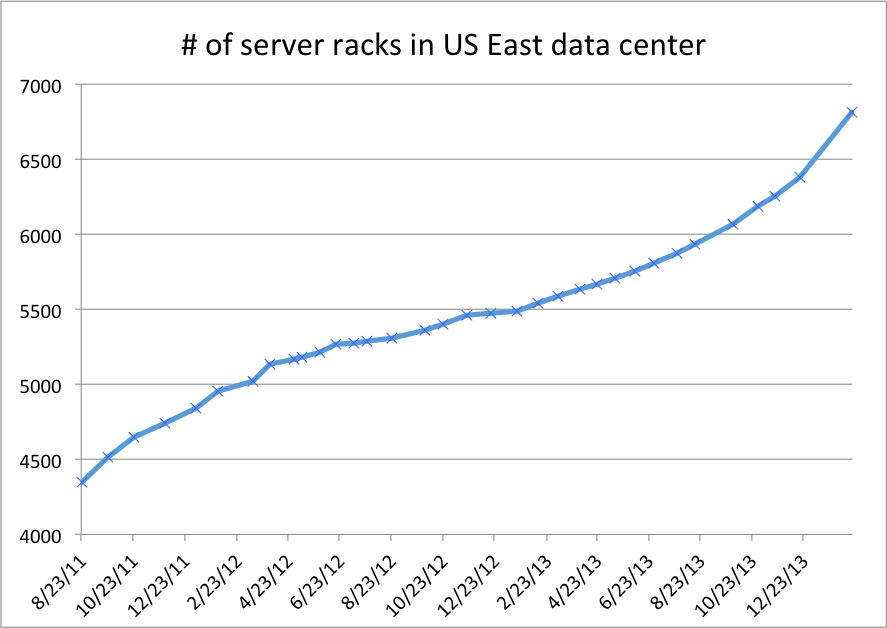
\includegraphics[width=.7\textwidth]{imagens/servidores.png}
\caption{Crescimento do número de servidores}
\label{servidores}
\end{figure}

Apesar desse crescimento exponencial, o custo não aumenta, uma vez que com o passar dos anos, novas tecnologias fazem com que o preço dos componentes diminua, como mostra a figura \ref{custo}.\\

\begin{figure}[H]
\centering
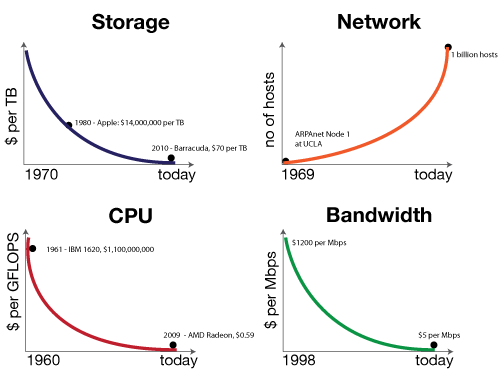
\includegraphics[width=.7\textwidth]{imagens/custo.png}
\caption{Queda do custo dos componentes}
\label{custo}
\end{figure}

Com toda a facilidade de expansão vem um custo. Este custo é relacionado com a perda de desempenho quando há subutilização da rede, ou seja, quanto maior e mais complexa a rede, mais difícil de gerenciar e com isso, há o aumento da latência. A figura \ref{capacity} mostra um pouco este desequilíbrio. A linha azul clara mosta a latência da rede e a linha azul escura mostra o número de servidores necessários para que a latência se mantenha constante com o aumento da quantidade de tráfego de dados.\\

\begin{figure}[H]
\centering
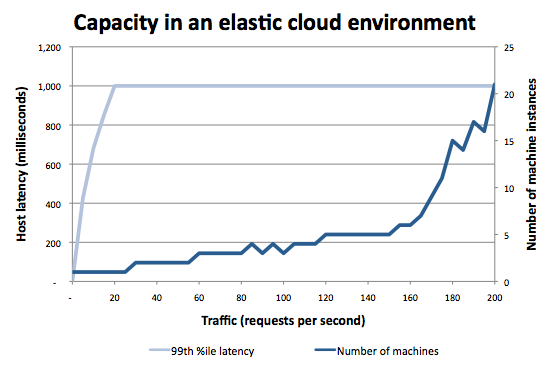
\includegraphics[width=.7\textwidth]{imagens/capacity.png}
\caption{Latência da rede x Aumento do tráfego}
\label{capacity}
\end{figure}

Com isso, as topologias e os protocolos são muito importantes para equilibrar todos os requisitos sem que haja perda de qualidade de serviço para o usuário. A seguir, vamos apresentar as topologias das redes de datacenters mais utilizadas.\\

\chapter{Topologias}
A seguir, mostraremos algumas topologias, algumas são mais escaláveis, outras mais redundantes, porém todas possuem vantagens e desvantagens.\\

\section{Tradicionais}
As topologias tradicionais são aquelas que são fisicamente montadas e necessitam manutenção de hardware.\\

\subsection{Baseadas em Árvores}
As topologias baseadas em árvores são as seguintes:\\
\begin{itemize}
\item Basic Tree
\item Fat-Tree
\item VL2 
\end{itemize}

\paragraph{Basic Tree}
A primeira estrutura hierárquica que foi pensada foi uma árvore básica, geralmente com 3 níveis, onde a raiz possui a tarefa de controlar os fluxos que entram e saem do datacenter. Os switches do segundo nível fazem a atribuição dos domínios, roteamento e balanceamento de carga. O terceiro nível é também responsável por um balanceamento de carga entre os servidores, mas em um nível menos. Além disso, este nível consegue controlar um pouco do congestionamento da rede.\\

A figura \ref{basic_tree} mostra o esquema básico para esta árvore de 3 níveis.\\

\begin{figure}[H]
\centering
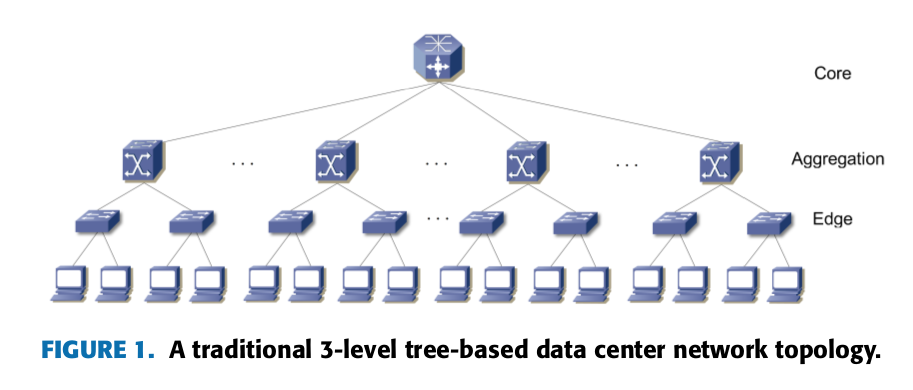
\includegraphics[width=.8\textwidth]{imagens/basic_tree.png}
\caption{Latência da rede x Aumento do tráfego}
\label{basic_tree}
\end{figure}

O crescimento do Oversubscription na direção do Core da rede pode causar alguns problemas, como por exemplo o incast, onde os servidores tentam transmitir ao mesmo tempo na direção do Core, isto causa um congestionamento na rede.\\

\paragraph{Fat-Tree}
Para tentar resolver os problemas da topologia anterior, foi desenvolvida a Fat-Tree, que possui mais do que um switch Core e possui conexões cruzadas na camada de agregação. Isso faz com que seja possível os servidores utilizarem vários caminhos diferentes até um switch Core. Esta ideia da redundância de caminhos vem para evitar o congestionamento da rede e tentar resolver o problema do incast que ocorria no caso anterior.\\

Além disso, é uma estrutura rearranjável não bloqueante e fornece uma relação de Oversubscription de 1:1 a todos os servidores. No entanto, a complexidade da fiação é O(n3), que é um desafio sério.\\

A figura \ref{fat_tree} mostra a topologia básica para uma fat-tree de 3 níveis.\\

\begin{figure}[H]
\centering
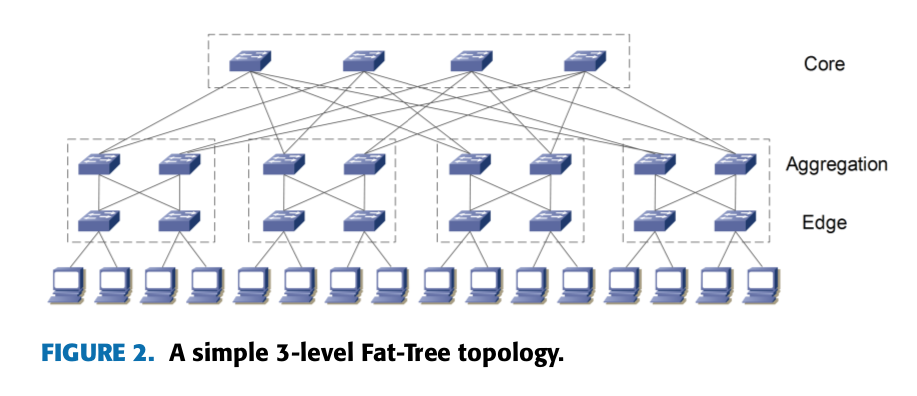
\includegraphics[width=.8\textwidth]{imagens/fat_tree.png}
\caption{Latência da rede x Aumento do tráfego}
\label{fat_tree}
\end{figure}

\paragraph{VL2}
Esta topologia possui switches em uma topologia de rede CLOS que Usa o VLB (Valiant Load Balancing) para distribuir tráfego entre os caminhos da rede. Além disso, usa uma modificação do protocolo ARP (Address Resolution Protocol) para que seja escalável para um número grande de servidores, onde o broadcast é feito somente na região local de cada servidor.\\

\subsection{Recursivas}
As topologias recursivas são as seguintes:\\
\begin{itemize}
\item Dcell
\item Bcube
\item FiConn
\item FlatNet
\item SprintNet
\end{itemize}

\paragraph{Dcell}
A topologia Dcell utiliza a ideia de células compostas por 1 switch e servidores conectados neste switch. As células são interligadas então através dos servidores com outras células. Assim, o número de células é limitado pelo número de portas do servidor. Esta topologia é meio limitada quanto à expansão, uma vez que para que haja a redundância de conexões, cada servidor está conectado com outro servidor em outra célula. Para expandir o número de células é necessário que haja uma troca do switch por outro com um número maior de portas.\\

Neste caso, o roteamento dentro da própria célula é feito pelo switch e o roteamento com outras células é feito pelos próprios servidores, o que causa um overhead e consequentemente um pequeno atraso do redirecionamento dos fluxos.\\

A figura \ref{dcell} mostra um exemplo desta topologia para switches com 4 portas.\\

\begin{figure}[H]
\centering
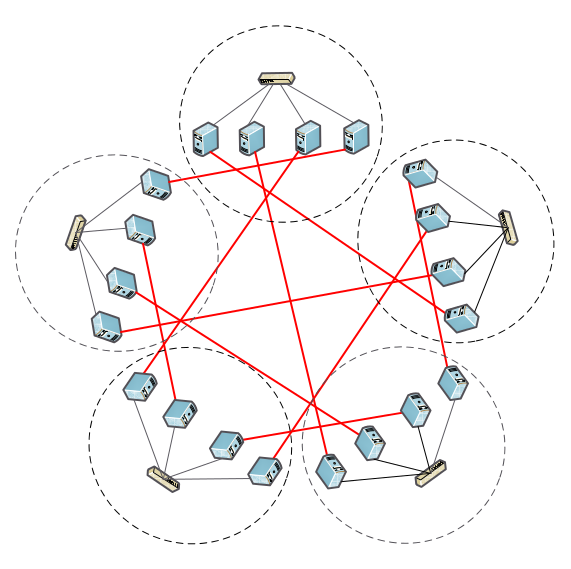
\includegraphics[width=.8\textwidth]{imagens/dcell.png}
\caption{Topologia Dcell para switches de 4 portas}
\label{dcell}
\end{figure}

\paragraph{Bcube}
Assim como no caso anterior, esta topologia se baseia na ideia de células interconectadas mas deixa a complexidade do redirecionamento dos fluxos para os switches, uma vez que neste caso, as células são conectadas por switches ao invés dos próprios servidores. Além disso, esta topologia também sofre limitações por conta do número de portas dos switches.\\

A figura \ref{bcube} mostra esta topologia com 3 níveis e switches de 4 portas.\\

\begin{figure}[H]
\centering
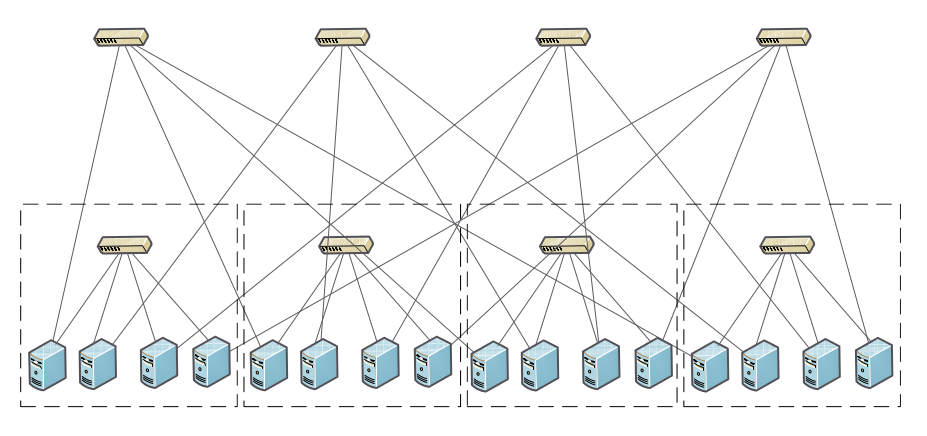
\includegraphics[width=.8\textwidth]{imagens/bcube.png}
\caption{Topologia Bcube para switches de 4 portas}
\label{bcube}
\end{figure}

\paragraph{FiConn}
Esta topologia é muito semelhante à Dcell, porém possui a limitação de ter somente 2 links conectados em cada célula, ou seja, diminui a complexidade de fios que esta topologia necessita. Porém, a capacidade da rede é diminuida, uma vez que menos links significam menos largura de banda e pode ser que ocorram congestionamentos mais facilmente.\\

A figura \ref{ficonn} mostra a topologia da rede.\\

\begin{figure}[H]
\centering
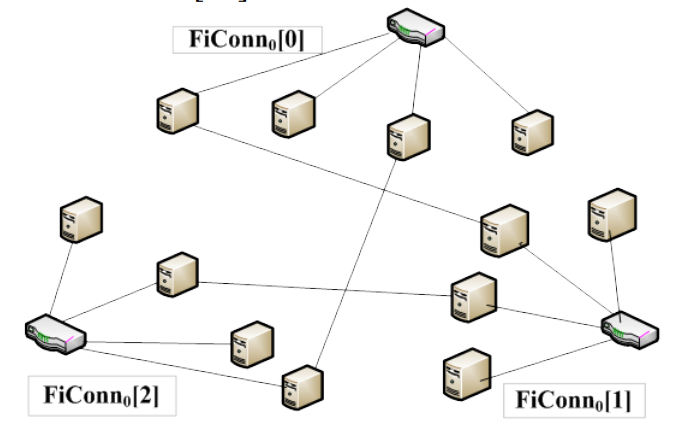
\includegraphics[width=.8\textwidth]{imagens/ficonn.png}
\caption{Topologia Bcube para switches de 4 portas}
\label{ficonn}
\end{figure}

\paragraph{FlatNet}
Esta topologia é semelhante ao Bcube, porém é mais interconectada, porque cada célula está conectada com $n$ switches, onde $n$ é o número de portas do switch interno da célula. A segunda camada de switches por sua vez conecta $n$ células. A diferença é que esta topologia divide a tarefa de roteamento com os switches e com os servidores, assim, os servidores podem rotear fluxos para outras células.\\

A figura \ref{flatnet} mostra esta topologia para $n=4$.\\

\begin{figure}[H]
\centering
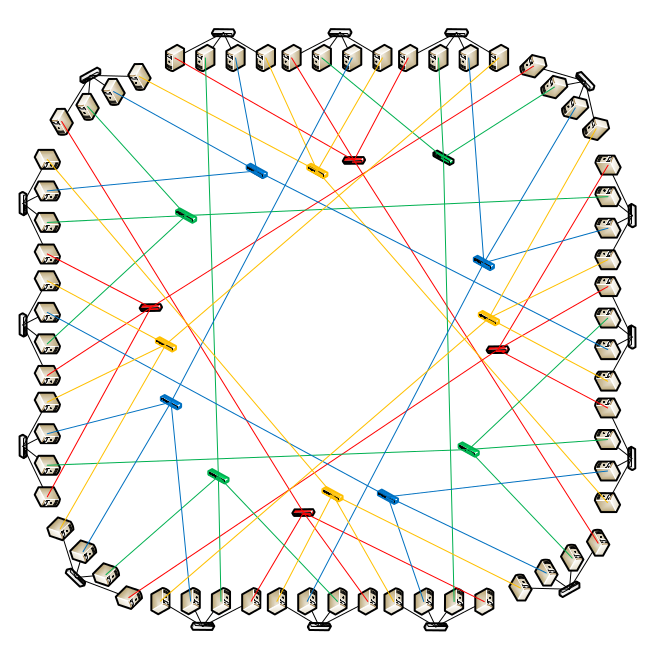
\includegraphics[width=.8\textwidth]{imagens/flatnet.png}
\caption{Topologia Bcube para switches de 4 portas}
\label{flatnet}
\end{figure}

\paragraph{SprintNet}
Esta topologia utiliza células com 2 switches e 4 servidores e existe uma redundância nas conexões internas da célula. Neste caso, todas as conexões entre células são feitas pelos servidores conectados com switches. Isso faz com que todo fluxo interno seja roteado pelo switch e o fluxo externo seja roteado tanto pelos switches como pelos servidores. Assim, existem diversos caminhos que podem ser utilizados para a comunicação inter-células.\\

A figure \ref{sprintnet} mostra esta topologia.\\

\begin{figure}[H]
\centering
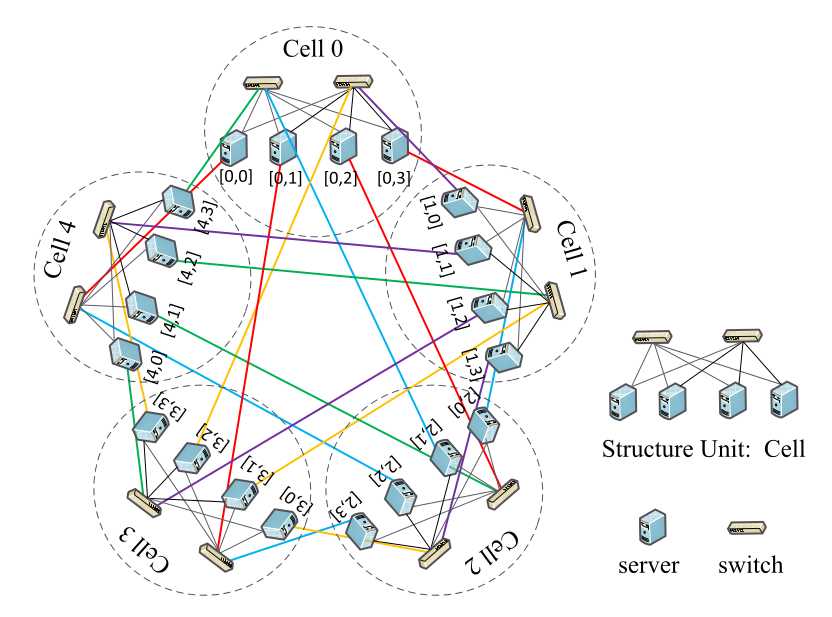
\includegraphics[width=.8\textwidth]{imagens/springnet.png}
\caption{Topologia Bcube para switches de 4 portas}
\label{sprintnet}
\end{figure}

A tabela da figura \ref{comparacao} mostra a comparação da complexidade de algumas topologias mostradas. Como pode ser visto, as redes que suportam o maior número de servidores, também possuem uma complexidade muito grande de conexões, o que aumenta a complexidade de roteamento mas também aumenta o número de caminhos que podem ser escolhidos para um fluxo.\\

\begin{figure}[H]
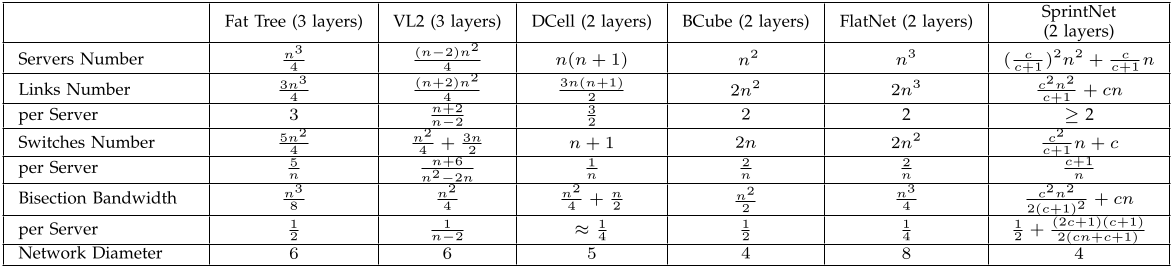
\includegraphics[width=1.1\textwidth]{imagens/tabela.png}
\caption{Topologia Bcube para switches de 4 portas}
\label{comparacao}
\end{figure}

\section{SDN}

\chapter{Protocolos}

\chapter{Tendências}

\chapter{Conclusão}

\chapter{Referências}

\begin{itemize}
\item Manual de referência do NS-3 \begin{verbatim}https://www.nsnam.org/docs/release/3.8/manual.pdf\end{verbatim}
\item Documentação \begin{verbatim}https://www.nsnam.org/doxygen/index.html\end{verbatim}
\end{itemize}

\end{document}
